\documentclass[serif, aspectratio=169]{beamer}
\setbeamertemplate{caption}{numbered}
\usecolortheme{dolphin}
%\usepackage{beamerthemesplit}
\usetheme{Frankfurt}
\usepackage{amssymb}
\usefonttheme{serif}
\setbeamertemplate{navigation symbols}{}


\usepackage[T1]{fontenc} 
\usepackage{fourier} % see "http://faq.ktug.org/wiki/uploads/MathFonts.pdf" for other options
\usepackage{hyperref}
\usepackage{latexsym,amsmath,xcolor,multicol,booktabs,calligra}
\usepackage{graphicx,pstricks,listings,stackengine}
\usepackage{lipsum}
\usepackage{lmodern}

\newcommand{\sd}{\partical\varphi}
\newcommand{\sdp}{\partial\phi}
\newcommand{\vp}{\varphi}
\newcommand{\lam}{\lambda}
\newtheorem{thm}{Theorem}
\newtheorem{thm co}{Theorem contd...}
\newtheorem{lem}{Lemma}
\newtheorem{Ass}{Asumption}
\newtheorem{Def}{Definition}
\newtheorem{remark}{Remark}
\usepackage{pifont}
\usepackage{mathrsfs,amsmath,amsfonts,amssymb}
\usepackage{graphicx,epstopdf,tikz}
%\usepackage{graphicx}
\usepackage{mathrsfs,amsmath}
\usepackage{subfigure,epstopdf}
\usepackage{array}
\usepackage{booktabs}
\usepackage{tikz}
\usetikzlibrary{positioning}

\title {Analyzing Diabetic Vulnerability to Emerging Viral Threats}
\author[]{\textbf{Under the guidance of}\\
\textcolor{blue}{Ms. R. NANDHINI M.Sc., SET, M.Phil., (Ph.D.)}\\
Assistant Professor\\
Department Of Mathematics (SF)\\
PSG College of Arts \& Science\\
Coimbatore}
\institute{\textbf{Presented by}\\
\textbf{\textcolor{red}{SIBIVENDHAN K - 23MMA132\\
SINEKA S - 23MMA133}}}
\date{\small \today}
 
% defs
\def\cmd#1{\texttt{\color{red}\footnotesize $\backslash$#1}}
\def\env#1{\texttt{\color{blue}\footnotesize #1}}
% set colors
\definecolor{hkustyellow}{RGB}{167, 131, 55}
\definecolor{hkustblue}{RGB}{0, 56, 116}
\definecolor{hkustred}{RGB}{209, 51, 59}

\lstset{
    basicstyle=\ttfamily\small,
    keywordstyle=\bfseries\color{deepblue},
    emphstyle=\ttfamily\color{deepred},    % Custom highlighting style
    stringstyle=\color{deepgreen},
    numbers=left,
    numberstyle=\small\color{halfgray},
    rulesepcolor=\color{red!20!green!20!blue!20},
    frame=shadowbox,
}



\begin{document}


\begin{frame}
    \titlepage
    \vspace*{-0.6cm}

\end{frame}

\begin{frame}
\begin{block}{TABLE OF CONTENTS}
    

\tableofcontents[sectionstyle=show,
subsectionstyle=show/shaded/hide,
subsubsectionstyle=show/shaded/hide]
\end{block}
\end{frame}

% Introduction --- --- --- --- --- --- -

\section{ABSTRACT}
\begin{frame}
\frametitle<presentation>{ABSTRACT}
\hspace{1em}This study aims to predict the age group most vulnerable to diabetes in the context of emerging viral threats. We employ and compare two decision-making techniques: Simple Additive Weighting (SAW) and Fuzzy Multiple Criteria Decision Making (MCDM) using the Technique for Order of Preference by Similarity to Ideal Solution (TOPSIS). Real time data on age, glucose levels, blood pressure, skin thickness, insulin, body mass index and diabetes pedigree function are collected to identify susceptible individuals. The research evaluates the effectiveness of both techniques and recommends the most suitable approach for prediction. Finally, the study offers recommendations for diabetes management based on the finding.   
\end{frame}

\section{INTRODUCTION}
\begin{frame}
\frametitle<presentation>{INTRODUCTION}
\begin{figure}
    \centering
    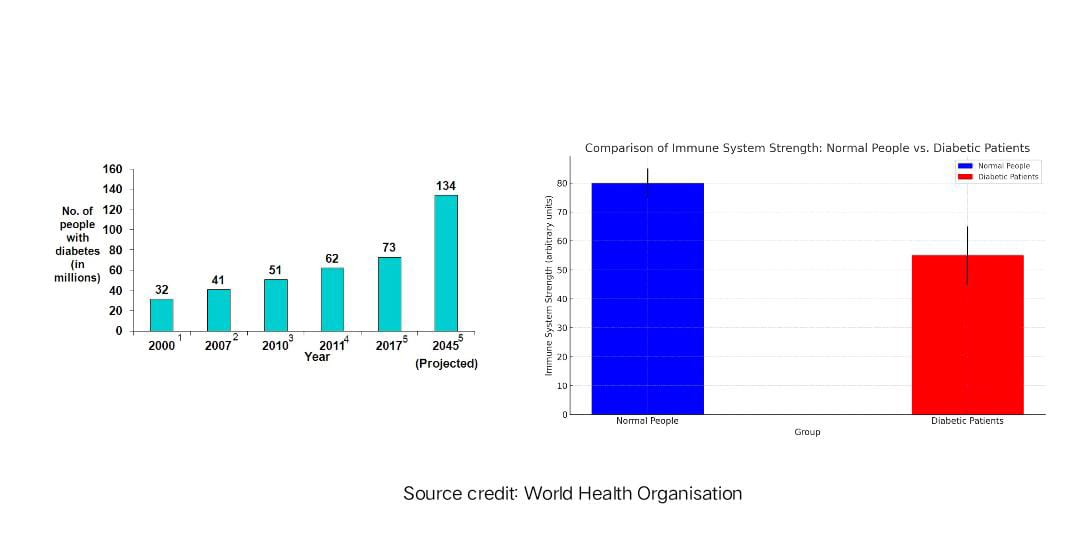
\includegraphics[width=1\textwidth]{intro.jpg}
\end{figure}
\end{frame}
\section{PRELIMINARIES}
\begin{frame}
\frametitle<presentation>{PRELIMINARIES}
\begin{block} {Definition 1: Fuzzy set}
\hspace{1em}A fuzzy set is any set that allows its members to have different grades of membership (membership function) in the interval [0,1]. 
\end{block}
\begin{block}{Definition 2: Membership function}
\hspace{1em}A numerical function between 0 and 1 that represents the degree to which an element belongs to a particular set, also referred to as membership value. The value 0 means that is not a member of the fuzzy set; the value 1 means that is fully a member of the fuzzy set. The values between 0 and 1 characterize fuzzy members, which belong to the fuzzy set only partially.
\end{block} 
\end{frame}
\begin{frame}{Fuzzy Logic}
    \begin{figure}
        \centering
        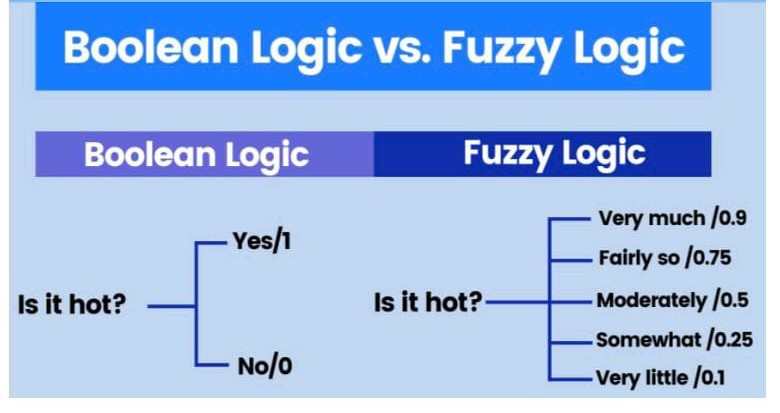
\includegraphics[width=0.5\linewidth,height=0.5\linewidth]{fuzzy.jpg}
    \end{figure}

\end{frame}

\begin{frame}
\frametitle<presentation>{PRELIMINARIES}
\begin{block} {Definition 3: MCDM}
\hspace{1em}It refers to a set of methods and processes used to evaluate and prioritize alternatives based on multiple, often conflicting, criteria. MCDM helps decision-makers identify the most suitable option among a set of alternatives by considering various factors simultaneously.
\end{block} 

\begin{block}{Definition 4: SAW}
\hspace{1em}It is a straightforward MCDM method used to evaluate and rank alternatives based on multiple criteria. It involves scoring each alternative on each criterion, then aggregating these scores using a weighted sum to produce an overall score for each alternative.
\end{block} 
\end{frame}
\begin{frame}
 \begin{block}{Definition 5: TOPSIS}      
\hspace{1em}It is a MCDM method that identifies the best alternative based on the shortest distance to an ideal solution and the farthest distance from an anti-ideal solution. The fundamental principle behind TOPSIS is that the chosen alternative should have the closest proximity to the ideal solution while being the farthest from the worst case scenario.
    \end{block}
   
\begin{block}{Definition 6: Fuzzy TOPSIS}

\hspace{1em}It is an extension of the traditional TOPSIS method that incorporates fuzzy logic to handle uncertainty and imprecision in decision-making. This approach is particularly useful when decision criteria are subjective or qualitative, allowing for a more nuanced evaluation of alternatives.
   \end{block} 
    
\end{frame}

\section{ANALYTICAL APPROACH }
\begin{frame}{Steps to solve SAW:}
\begin{enumerate}
\item \textbf{The initial matrix is prepared based on the values for m$\times$n matrix $r_{ij}$ is the value of the $i^{th}$ criterion for $j^{th}$ object where:}
\vspace{3mm}
\begin{itemize}
    \item i = 1,2,...,m;
    \vspace{1mm}
    \item j = 1,2,...,n;
\end{itemize}
\vspace{3mm}
\hspace{1em}Another point is to determine the weights of the criteria ($w_{i}$) to show their importance. These weights can be considered as numbers between zero and one (or by percentages) and considering $\sum\limits^{n}_{i\text{=}1}w_{i}\text{=}1$\\
\end{enumerate}
\end{frame}

\begin{frame}
    \begin{enumerate}
\item \textbf{Normalizing the Value of $i^{th}$ Criterion for the $j^{th}$ Alternative:}\\ 
\hspace{1em}The $\overline{r_{ij}}$ is known as the normalized $i^{th}$ criterion’s value for $j^{th}$ alternative or object.\\
\vspace{-7mm}
\begin{eqnarray*}
\overline{r_{ij}}&\text{=}&\frac{\min (r_{ij})}{r_{ij}} ; \text{if j is a cost attribute.}\\
\overline{r_{ij}}&\text{=}&\frac{r_{ij}}{\max(r_{ij})} ; \text{if j is a benefit or profit attribute.}
\end{eqnarray*}\\
\vspace{-2mm}
\hspace{1em}where $r_{ij}$ is the value of the $i^{th}$ criterion for $j^{th}$ object. The $\max (r_{ij})$ is the largest value of the $i^{th}$ criterion when all alternatives are compared, and $\min (r_{ij})$ is the smallest value for it. Therefore,
 $\overline{r_{ij}}$ is a normalized value for the $i^{th}$ criterion and $j^{th}$
alternative.\\
\end{enumerate}
\end{frame}

\begin{frame}
\begin{enumerate}

\item \textbf{Sum up Values of the Criteria and Weights:}\\
\hspace{1em}The summation of the criteria and weights helps
to gain a single magnitude that is the final performance value for each alternative. For this, the following equation can be used for the $j^{th}$ alternative or object:\\
\vspace{2mm}
\begin{center}
    $S_{j}\text{=}\sum\limits^{n}_{n\text{=}1}w_{i}\overline{r_{ij}}$
\end{center}
\vspace{3mm}
\item \textbf{Ranking the Alternatives to Choose the
Best One:}\\
\hspace{1em}In the final step, the best alternative is chosen
based on the largest performance value of the $S_{j}$ \maximizing criterion, and the smallest for the minimizing criterion\\
\vspace{3mm}
\hspace{1em}The $r_{ij}$ is this method should be positive. According to this requirement the negative values should be transferred to positive ones $(\overline r_{ij})$ using different methods. For example, the following formula can be used:\\
\begin{center}
   $\overline r_{ij} \text{=} r_{ij} $+$ |{\min (r_{ij})}|\text{+}1$
    
\end{center}
\vspace{2mm}
\end{enumerate}
\end{frame}

\begin{frame}{SAW outcome}

\begin{figure}
    \centering
    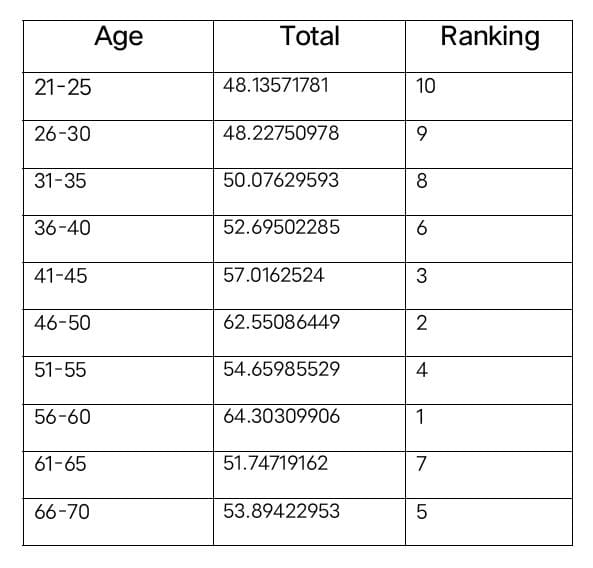
\includegraphics[width=0.7\linewidth,height=0.38\textwidth]{total.jpg}

\end{figure}
  
  \hspace{1em} From the above outcome we observe that the age category between 56-60 are the most susceptible diabetic patients for the emerging viral threats. 
\end{frame}

\begin{frame}{Visualization}
    \begin{figure}
        \centering
        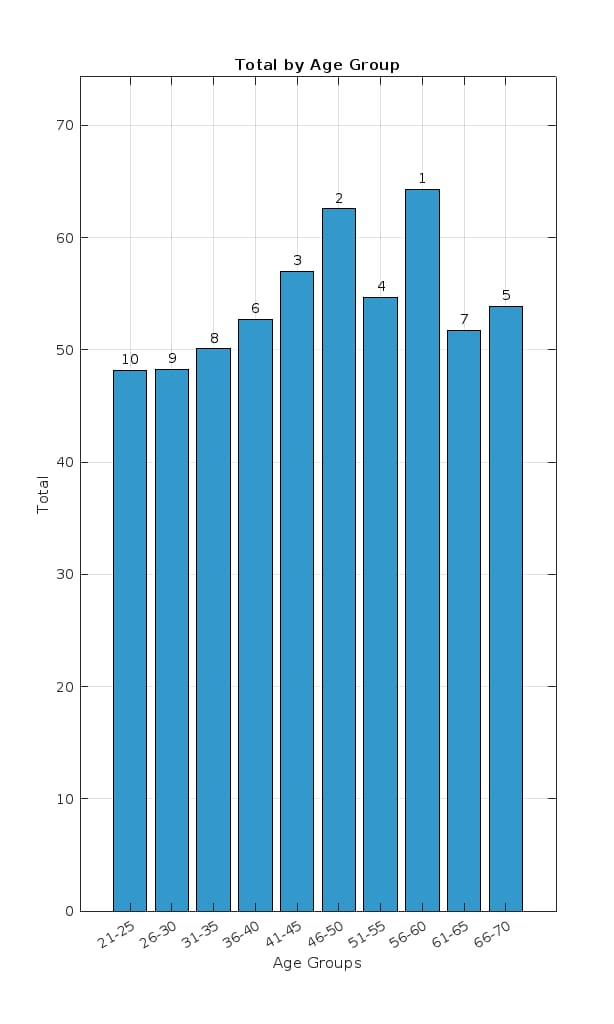
\includegraphics[width=0.6\linewidth,height=0.55\linewidth]{matlab_1.jpg}

    \end{figure}
\end{frame}

\begin{frame}{Steps to solve TOPSIS}
\begin{itemize}
    \item \textbf{Normalize the decision matrix:}
     \vspace{-5mm}
    \begin{center}
\begin{eqnarray*}
    r_{ij}&\text{=}&\frac{x_{ij}}{\sqrt{\sum\limits^{m}_{k\text{=}1}x^{2}_{kj}}},
    \hspace{2mm}\text{i=1,2,...,m;} \hspace{2mm} \text{j=1,2,...,n;}
 \end{eqnarray*}   
    \end{center}
\hspace{1em}Multiply the columns of normalized decision matrix by the associated weights:
\vspace{-1cm}
\begin{center}
\begin{eqnarray*}
v_{ij}&\text{=}& w_{i} \times  r_{ij},\hspace{2mm}\text{i=1,2,...,m; \hspace{2mm} j=1,2,...,n;}
\end{eqnarray*}
\end{center}

\item \textbf{Determine the positive ideal and negative ideal solutions:} 
\vspace{-1.5cm}
\begin{center}
\begin{eqnarray*}

    A^{\text{+}}&\text{=}& \{v^{\text+}_{1}, v^{\text+}_{2},...,v^{\text+}_{n}\} \text= \{(\max(v_{ij})|j\in K_{b}) (\min(v_{ij})|j \in K_{c})\} 

    A^{-} &\text{=}& \{v^{-}_{1}, v^{-}_{2},...,v^{-}_{n}\} \text= \{(\min(v_{ij})|j\in K_{b}) (\max(v_{ij})|j \in K_{c})\} 
     
\end{eqnarray*} 
\end{center}
\vspace{-1.5cm}
\hspace{1em}where $K_{b}$ is a set of benefit criteria and $K_{c}$ is a set of cost criteria.
\end{itemize}
\end{frame}
\begin{frame}
\begin{itemize}
\item \textbf{Obtain the distances of the existing alternatives from the positive ideal and negative ideal solutions:} \\
\hspace{1em}Two Euclidean distances for each alternatives are, respectively, calculated as follows:
\begin{center}
$S_{i}^{\text+}\text=\sqrt{\sum\limits_{j\text=1}^{n}(v_{ij}-v_{j}^{\text+}})^{2}$, i= 1,2,...,m\\
$S_{i}^{-}\text=\sqrt{\sum\limits_{j\text=1}^{n}(v_{ij}-v_{j}^{-}})^{2}$, i= 1,2,...,m 
\end{center}
\vspace{2mm}
\item \textbf{Calculate the relative closeness to the ideal alternatives:} 
\begin{center}
\vspace{2mm+}
$RC_{i}\text=\frac{S_{i}^{-}}{S_{i}^{\text+}\text+S^{-}_{i}}$ ;i= 1, 2, ... , m; $0\leq RC_{i}\leq 1$    
\end{center}
\vspace{2mm}
\item \textbf{Rank the alternatives according to their relative closeness to the ideal alternatives.}
\end{itemize}   
\end{frame}

\begin{frame}{Steps to solve Fuzzy MCDM(TOPSIS)}
\begin{itemize}
  
    \item \textbf{Normalizing the decision matrix:}\\
\hspace{1em}An appropriate and methodologically justified method for normalization of fuzzy decision matrices was developed in as follows:
\begin{center}
$\overline{r_{ij}}\text=(r_{ij}^{L},r_{ij}^{M},r_{ij}^{U})\text=(\frac{a_{ij}}{c_{j}^{\text+}},\frac{b_{ij}}{c_{j}^{\text+}},\frac{c_{ij}}{c_{j}^{\text+}})$;i=1,...,m;$j \in K_{b}$,
   
\end{center}

\hspace{1em}where $c^{\text+}_{j}\text=\max_{i}(c_{ij});j \in K_{b}$.

\begin{center}

$\overline{r_{ij}}\text=(r_{ij}^{L},r_{ij}^{M},r_{ij}^{U})\text=(\frac{a_{ij}}{c_{j}^{-}},\frac{b_{ij}}{c_{j}^{-}},\frac{c_{ij}}{c_{j}^{-}})$;i=1,...,m;$j \in K_{c}$,
    
\end{center}
\hspace{1em}where $a^{\text+}_{j}\text=\min_{i}(a_{ij});j \in K_{c}$.
This normalization guarantees that $\overline{r_{ij}}\subset [0,1]$ for all i and j.
\end{itemize}
\end{frame}

\begin{frame}
\begin{itemize}
    
\item \textbf{The positive and negative ideal solutions are obtained as follows:}
\vspace{3mm}


$$A^{\text+}\text=\{\overline{r^{\text+}_{1}},\overline{r^{\text+}_{2}},...,\overline{r^{\text+}_{n}}\}\text=\{ \max\{(r_{ij}^{L},r_{ij}^{M},r_{ij}^{U})\}|j\in K_{b}, \min\{(r_{ij}^{L},r_{ij}^{M},r_{ij}^{U})\}|j\in K_{c}\},$\\
\vspace{3mm}

$$A^{-}\text=\{\overline{r^{-}_{1}},\overline{r^{-}_{2}},...,\overline{r^{-}_{n}}\}\text=\{ \min\{(r_{ij}^{L},r_{ij}^{M},r_{ij}^{U})\}|j\in K_{b}, \max\{(r_{ij}^{L},r_{ij}^{M},r_{ij}^{U})\}|j\in K_{c}\},$$

 \vspace{3mm}
 \item \textbf{Calculation of separation of each alternative from the positive and negative ideal solutions:}\\
\vspace{2mm}
\begin{center}

$\overline{r_{j}^{\text+}} \geq \overline{r_{ij}} ,\hspace{1mm} i\text=1,2...m ,\hspace{1mm} j \in K_{b}$

$\overline{r_{ij}} \geq \overline{r_{j}^{\text+}} ,\hspace{1mm} i\text=1,2...m ,\hspace{1mm} j \in K_{c}$

$\overline{r_{ij}} \geq \overline{r_{j}^{-}} ,\hspace{1mm} i\text=1,2...m ,\hspace{1mm} j \in K_{b}$

$\overline{r_{j}^{-}} \geq \overline{r_{ij}} ,\hspace{1mm} i\text=1,2...m ,\hspace{1mm} j \in K_{c}$
    
\end{center}
\end{itemize}
\end{frame}


\begin{frame}

\hspace{1em}Therefore, there is no need to use n-dimensional Euclidean or Hamming distances for obtaining $S_{i}^{\text+}$ and $S_{i}^{-}$ i = 1, 2,..., m, as they can be calculated as follows:
\vspace{-5mm}

\begin{center}
    
\begin{eqnarray*}
S_{i}^{\text+}&\text=&\sum_{j \in K_{b}}w_{j}(\overline{r_{j}^{\text+}}-\overline{r_{ij}})\text+\sum_{j \in K_{c}}w_{j}(\overline{r_{ij}}-\overline{r_{j}^{\text+}}),\\
S_{i}^{-}&\text=&\sum\limits_{j \in K_{b}}w_{j}(\overline{r_{ij}}-\overline{r_{j}^{-}})\text+\sum\limits_{j \in K_{c}}w_{j}(\overline{r_{j}^{-}}-\overline{r_{ij}})

\end{eqnarray*}

\end{center}
\vspace{-8mm}
\hspace{1em}These expressions make it possible to look at the problem from another point of view.

\begin{center}

$\overline{r_{j}^{\text+}} - \overline{r_{ij}} , \vspace{1mm}i\text=1,2...m , \vspace{1mm} j \in K_{b}$

$\overline{r_{ij}} - \overline{r_{j}^{\text+}} , \vspace{1mm} i\text=1,2...m , \vspace{1mm} j \in K_{c}$

$\overline{r_{ij}} - \overline{r_{j}^{-}} ,\vspace{1mm} i\text=1,2...m , \vspace{1mm}j \in K_{b}$

$\overline{r_{j}^{-}} - \overline{r_{ij}} ,\vspace{1mm}i\text=1,2...m ,\vspace{1mm} j \in K_{c}$
    
\end{center}
    
\end{frame}


\begin{frame}{Fuzzy outcome}
\begin{figure}
    \centering
    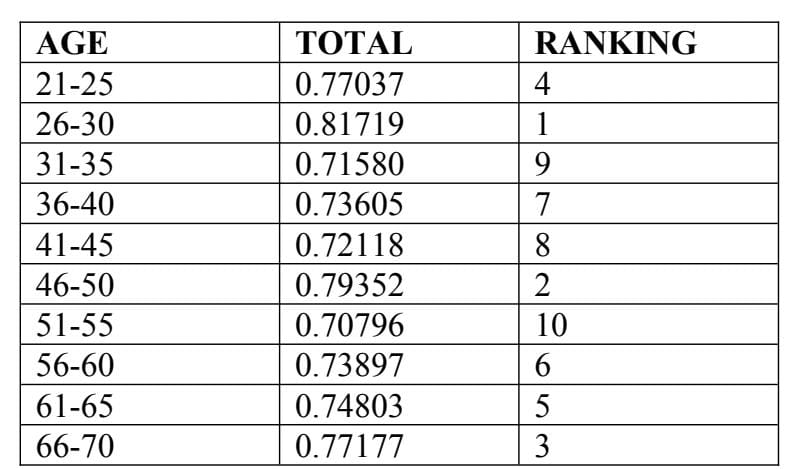
\includegraphics[width=0.5\linewidth]{fuzzy outcome.jpg}
\end{figure}
    \hspace{1em}From the above outcome we observe that the age category between 26-30 are the most susceptible diabetic patients for the emerging viral threats.
\end{frame}
\begin{frame}{Visualization 
}
\begin{figure}
    \centering
    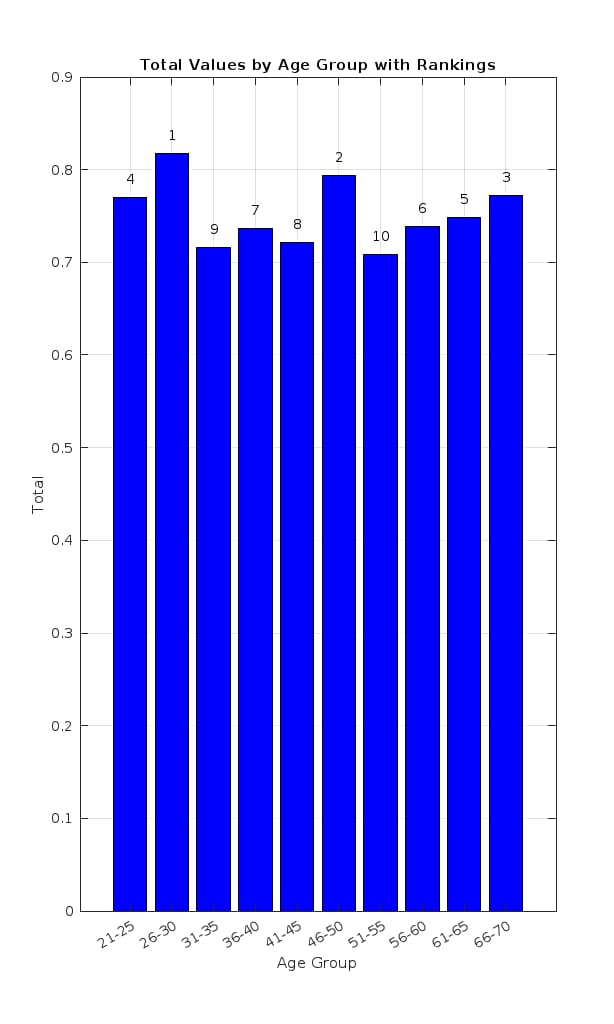
\includegraphics[width=0.6\linewidth,height=0.55\linewidth]{matlab_2.jpg}
\end{figure}
    
\end{frame}


\begin{frame}{Python}
    \begin{figure}
        \centering
        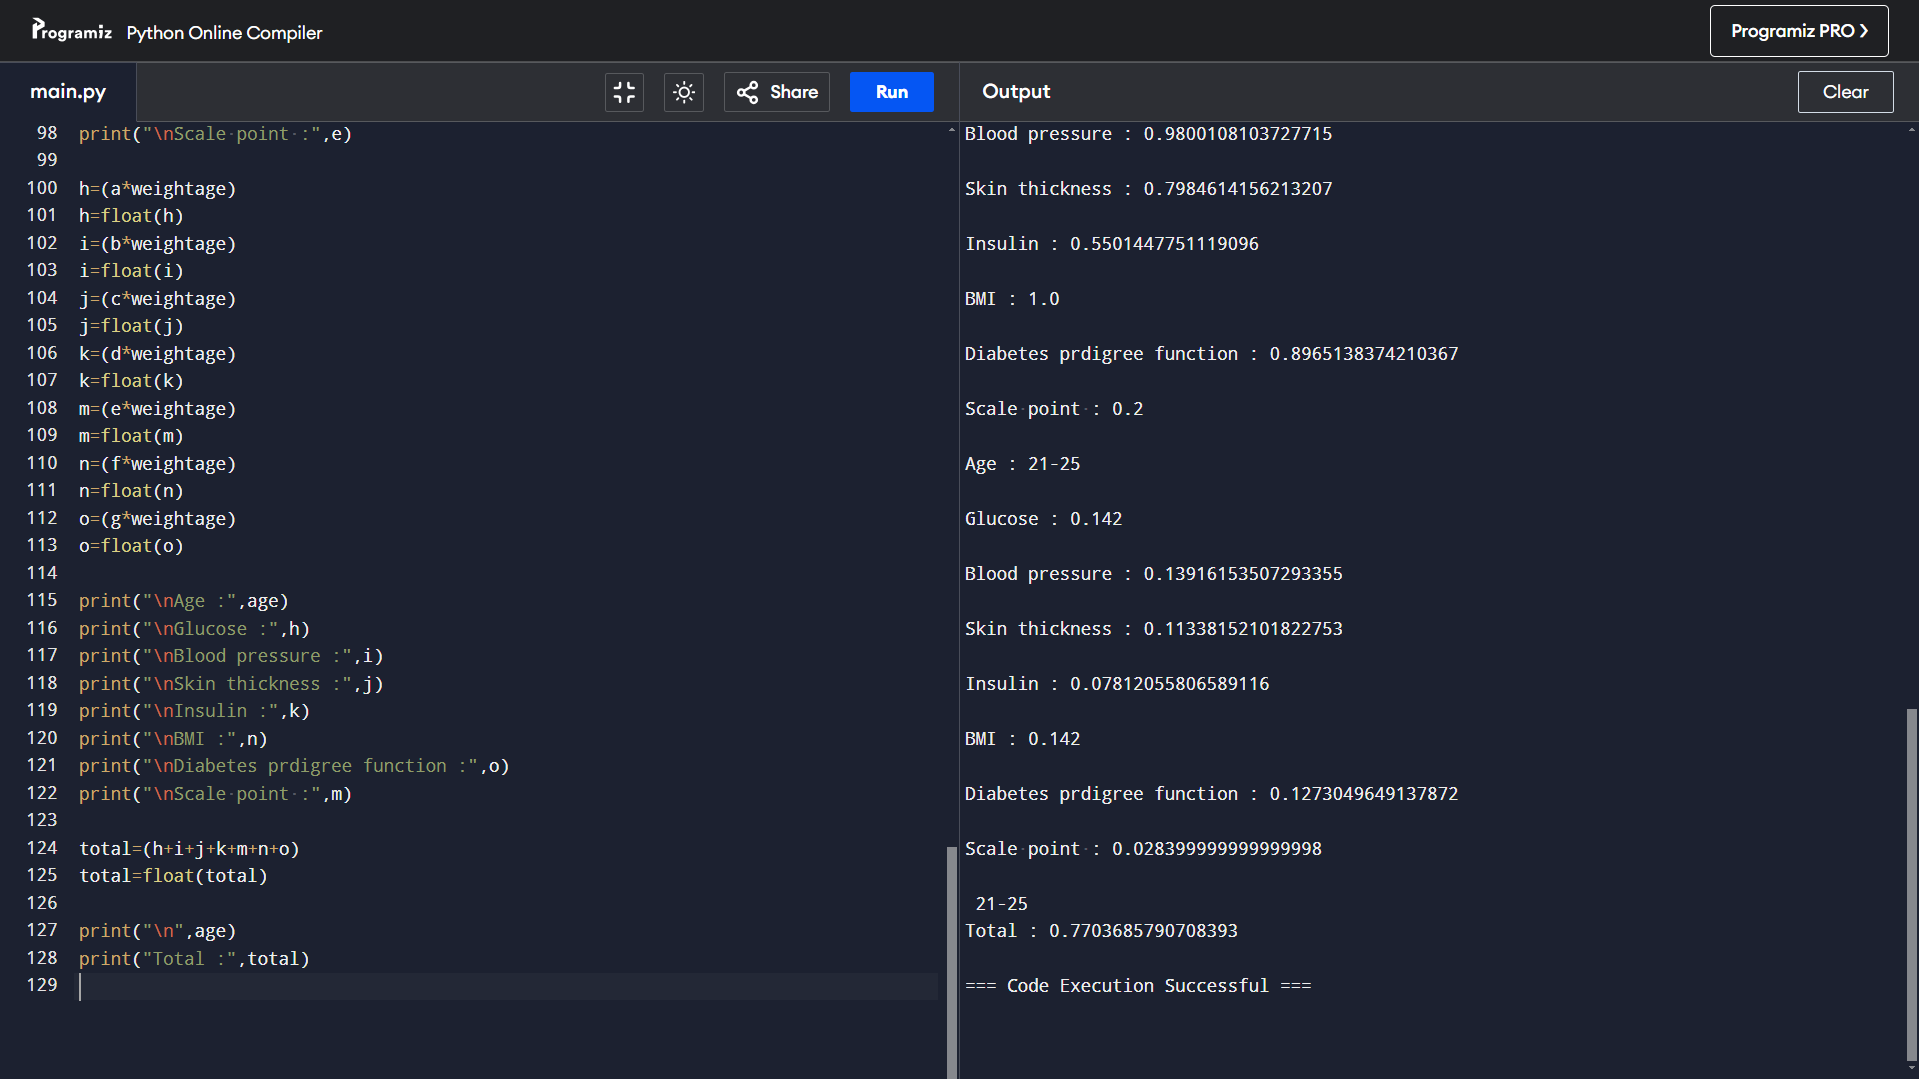
\includegraphics[width=1\linewidth]{Phyton .png}
    \end{figure}
\end{frame}

\section{COMPARISION}
\begin{frame}{COMPARISION OF SAW AND FUZZY TOPSIS:}
    
\textbf{Methodology:}
    \begin{itemize}
        \item \textbf{SAW :} This method aggregates scores of alternatives across multiple criteria by summing the weighted normalized scores. It is straightforward and easy to implement.

        \item \textbf{Fuzzy TOPSIS :} This method evaluates alternatives based on their distance from an ideal solution. It incorporates fuzzy logic to handle uncertainty and imprecision in data.
        \end{itemize}
\textbf{Handling Uncertainty:}
    \begin{itemize}
  
         \item \textbf{SAW: } While it can use fuzzy numbers, it generally requires precise values for the decision matrix, making it less effective in environments with high uncertainty.

        \item \textbf{Fuzzy TOPSIS: } Specifically designed to manage fuzzy data, it effectively incorporates uncertainty, making it more suitable for applications where data may be imprecise, such as predicting diabetic vulnerability.  
        
    \end{itemize}
\end{frame}

\begin{frame}
\item \textbf{Decision Criteria:}
    \begin{itemize}
        \item \textbf{SAW: } Requires clearly defined criteria and works well when these criteria are independent. It may struggle with interrelated criteria..

        \item \textbf{Fuzzy TOPSIS: } Can handle correlated criteria more efficiently by comparing the distance to both the ideal and negative-ideal solutions, allowing for more nuanced decision-making.  
 
    \end{itemize}

     \item \textbf{Application Suitability:}
    \begin{itemize}
        \item \textbf{SAW: } Best suited for simpler problems with well-defined metrics. It may provide quick results but can overlook subtleties in complex scenarios.

        \item \textbf{Fuzzy TOPSIS: } More appropriate for complex decision-making situations like assessing diabetic vulnerability where multiple overlapping factors and uncertainties exist.
 
    \end{itemize}
    
\end{frame}

\begin{frame}{Suggested Method for Predicting Diabetic Vulnerability}
\hspace{1em}Given the complexities involved in assessing diabetic vulnerability in the context of emerging viral threats, \textbf{Fuzzy TOPSIS} is recommended. Its ability to manage uncertainty, evaluate interrelated criteria, and provide a robust ranking of alternatives makes it more effective for this application. By incorporating fuzzy logic, the method can accommodate the varying degrees of risk associated with different factors, leading to more accurate and informed decision-making.
    
\end{frame}

\begin{frame}{Suggestions to Control \&  Prevent}
    1. Nutritional Strategies\\
	\qquad	a. Balanced Diet\\
	\qquad	b. Nutritional Supplements\\
2. Regular Physical Activity\\
3. Stress Management and Mental Well-being\\
	\qquad	a. Meditation and Mindfulness\\
	\qquad	b. Yoga \\
4. Sleep Hygiene\\
5. Preventive Healthcare Measures\\
6. Hygiene Practices\\
7. Educating and Empowering Patients\\
8. Healthy Snacking\\

\end{frame}
\section{CONCLUSION}
\begin{frame}{CONCLUSION}
\hspace{1em}This project demonstrates the effectiveness of integrating SAW and Fuzzy TOPSIS methodologies to assess the vulnerability of specific age groups to diabetes in the
context of emerging viral threats. By analyzing real-time health data, critical metrics
influencing susceptibility were identified, enhancing decision-making accuracy in public
health contexts. The comparative analysis revealed the respective strengths of these
techniques, with Fuzzy TOPSIS emerging as the superior method for this type of analysis. Further the development of software using Python code has significantly expedited
the generation of results, enabling swift predictions. This project not only contributes
to the field of public health but also offers a robust framework for decision-making across
diverse sectors, emphasizing the far-reaching impact of interdisciplinary approaches in
addressing contemporary challenges.
\end{frame}

\section{REFERENCE}
 \begin{frame}{REFERENCE}
\begin{itemize}

\bibitem{}
American Diabetes Association,
\textit{Standards of Medical Care in Diabetes – 2024}.
American Diabetes Association, January 2024, 45-68.

\bibitem{}
Bagh Ali,
\textit{Generalized Fuzzy TOPSIS to Solve Multi-Criteria Decision-Making Problems}, Journal of new theory 2020, 44-54.

\bibitem{}
Chen C.T., 
\textit{Extensions of The TOPSIS for Group Decision-Making under Fuzzy Environment}, Fuzzy Sets and Systems 114(1) (2020) 1-9.

\bibitem{}
Chen S. M., 
\textit{Fuzzy sets and fuzzy logic: A historical perspective}.
IEEE, 1996, 1-6.

\bibitem{}
Hamed Taherdoost, 
\textit{Analysis of Simple Additive Weighting Method (SAW) as a MultiAttribute Decision-Making Technique: A Step-by-Step Guide}.
Journal of Management Science \& Engineering Research, Volume 6, March 2023.


 \end{itemize}
 \end{frame}


\begin{frame}
\begin{itemize}
\bibitem{}
Hwang, C. L., \& Yoon, K., 
\textit{Multiple Attribute Decision Making: Methods and Applications}.
Springer-Verlag, 1981, 58-61, 99-116.

\bibitem{}
Lavanya, P., 
\textit{Multiple Attribute Decision Making: Methods and Applications}.
Springer-Verlag, 1981, 58-61.

\bibitem{}
Lutz, M., 
\textit{Learning Python}.
O'Reilly Media, 5th Edition, 2013, 1-30, 100-120.

\bibitem{}
McCance, 
\textit{Diabetes: A Comprehensive Guide}.
Wiley-Blackwell, 3rd edition, 2018, 15-45.

\bibitem{}
 Peter I. Kattan
\textit{MATLAB for Beginners: A Gentle Approach}.
Petra Books, 2008.


\end{itemize}     
 \end{frame}

 
\begin{frame}
\begin{center}
       {\Huge THANK YOU} 
\end{center} 
\end{frame}
\end{document}

